\documentclass[12pt]{article}\usepackage[]{graphicx}\usepackage[]{color}
%% maxwidth is the original width if it is less than linewidth
%% otherwise use linewidth (to make sure the graphics do not exceed the margin)
\makeatletter
\def\maxwidth{ %
  \ifdim\Gin@nat@width>\linewidth
    \linewidth
  \else
    \Gin@nat@width
  \fi
}
\makeatother

\definecolor{fgcolor}{rgb}{0.345, 0.345, 0.345}
\newcommand{\hlnum}[1]{\textcolor[rgb]{0.686,0.059,0.569}{#1}}%
\newcommand{\hlstr}[1]{\textcolor[rgb]{0.192,0.494,0.8}{#1}}%
\newcommand{\hlcom}[1]{\textcolor[rgb]{0.678,0.584,0.686}{\textit{#1}}}%
\newcommand{\hlopt}[1]{\textcolor[rgb]{0,0,0}{#1}}%
\newcommand{\hlstd}[1]{\textcolor[rgb]{0.345,0.345,0.345}{#1}}%
\newcommand{\hlkwa}[1]{\textcolor[rgb]{0.161,0.373,0.58}{\textbf{#1}}}%
\newcommand{\hlkwb}[1]{\textcolor[rgb]{0.69,0.353,0.396}{#1}}%
\newcommand{\hlkwc}[1]{\textcolor[rgb]{0.333,0.667,0.333}{#1}}%
\newcommand{\hlkwd}[1]{\textcolor[rgb]{0.737,0.353,0.396}{\textbf{#1}}}%
\let\hlipl\hlkwb

\usepackage{framed}
\makeatletter
\newenvironment{kframe}{%
 \def\at@end@of@kframe{}%
 \ifinner\ifhmode%
  \def\at@end@of@kframe{\end{minipage}}%
  \begin{minipage}{\columnwidth}%
 \fi\fi%
 \def\FrameCommand##1{\hskip\@totalleftmargin \hskip-\fboxsep
 \colorbox{shadecolor}{##1}\hskip-\fboxsep
     % There is no \\@totalrightmargin, so:
     \hskip-\linewidth \hskip-\@totalleftmargin \hskip\columnwidth}%
 \MakeFramed {\advance\hsize-\width
   \@totalleftmargin\z@ \linewidth\hsize
   \@setminipage}}%
 {\par\unskip\endMakeFramed%
 \at@end@of@kframe}
\makeatother

\definecolor{shadecolor}{rgb}{.97, .97, .97}
\definecolor{messagecolor}{rgb}{0, 0, 0}
\definecolor{warningcolor}{rgb}{1, 0, 1}
\definecolor{errorcolor}{rgb}{1, 0, 0}
\newenvironment{knitrout}{}{} % an empty environment to be redefined in TeX

\usepackage{alltt}

\input 4mbapreamble
\usepackage{amsfonts}
\usepackage{tikz}
\usetikzlibrary{shapes.geometric, arrows}
\tikzset{
  int/.style={circle, draw=black, fill=blue!20, minimum size=3em},
  init/.style={pin distance=1.2cm,pin edge={loop,thin,black}}
}
\tikzstyle{arrow} = [thick,black,->,>=stealth]
\tikzstyle{pinstyleto} = [pin edge={<-,thick,black}]
\tikzstyle{pinstyleout} = [pin edge={->,thick,black}]

%%%%%%%%%%%%%%%%%%%%%%%%%%%%%%%%%%%
%% FANCY HEADER AND FOOTER STUFF %%
%%%%%%%%%%%%%%%%%%%%%%%%%%%%%%%%%%%
\usepackage{fancyhdr,lastpage}
\pagestyle{fancy}
\fancyhf{} % clear all header and footer parameters
%%%\lhead{Student Name: \theblank{4cm}}
%%%\chead{}
%%%\rhead{Student Number: \theblank{3cm}}
%%%\lfoot{\small\bfseries\ifnum\thepage<\pageref{LastPage}{CONTINUED\\on next page}\else{LAST PAGE}\fi}
\lfoot{}
\cfoot{{\small\bfseries Page \thepage\ of \pageref{LastPage}}}
\rfoot{}
\renewcommand\headrulewidth{0pt} % Removes funny header line
%%%%%%%%%%%%%%%%%%%%%%%%%%%%%%%%%%%
\IfFileExists{upquote.sty}{\usepackage{upquote}}{}
\begin{document}

\begin{center}
{\bf Mathematics 4MB3/6MB3 Mathematical Biology\\
\smallskip
2016 ASSIGNMENT \textcolor{blue}{4}}\\
\medskip
\underline{\emph{Group Name}}: \texttt{{\color{blue}Model Students}}\\
\medskip
\underline{\emph{Group Members}}: {\color{blue}Nicole Dumont, Melody Fong, Carolina Weishaar}
\end{center}

\bigskip
\noindent
\textcolor{blue}{This assignment was due on Monday 13 March 2017 at 11:30am.}

\bigskip

\section{Time Series analysis of Recurrent Epidemics}

\begin{enumerate}[(a)]

\item You should have received the following data files by e-mail:
\begin{center}
\verb|meas_uk__lon_1944-94_wk.csv|\\
\verb|meas_uk__lpl_1944-94_wk.csv|
\end{center}
These plain text comma-separated-value files list weekly cases of
measles (in London and Liverpool, England, from 1944 to 1994).  Depending on which research direction you select, you might receive other files in the same \code{ymdc} (year,month,day,count) format, where the count column might contain cases or deaths, for example.  Write the following \Rlogo functions:

\begin{enumerate}[(i)]

\item \magcode{read.ymdc()}.  Read a file in \code{ymdc} format and
  return a data frame containing these data and including a
  \code{date} column that has \Rlogo's \magcode{Date} class.  The
  first (and potentially only) argument to this function should be the
  \code{filename} of the data file to be read.
  
{\color{blue}
\begin{proof}[Solution]
{\color{magenta}
\begin{knitrout}
\definecolor{shadecolor}{rgb}{0.969, 0.969, 0.969}\color{fgcolor}\begin{kframe}
\begin{alltt}
\hlstd{read.ymdc} \hlkwb{<-} \hlkwa{function}\hlstd{(}\hlkwc{filename}\hlstd{)\{}
  \hlstd{data} \hlkwb{<-} \hlkwd{read.csv}\hlstd{(filename,} \hlkwc{skip}\hlstd{=}\hlnum{6}\hlstd{)}
  \hlstd{ymdcdata} \hlkwb{<-} \hlkwa{NULL}

  \hlstd{ymdcdata}\hlopt{$}\hlstd{date} \hlkwb{<-} \hlkwd{as.Date}\hlstd{(}\hlkwd{paste}\hlstd{(}\hlkwd{as.character}\hlstd{(data}\hlopt{$}\hlstd{year),} \hlkwd{as.character}\hlstd{(data}\hlopt{$}\hlstd{month),}\hlkwd{as.character}\hlstd{(data}\hlopt{$}\hlstd{day),} \hlkwc{sep} \hlstd{=} \hlstr{"-"}\hlstd{))}
  \hlstd{ymdcdata}\hlopt{$}\hlstd{cases} \hlkwb{<-} \hlstd{data}\hlopt{$}\hlstd{cases}
  \hlstd{ymdcdata} \hlkwb{<-} \hlkwd{as.data.frame}\hlstd{(ymdcdata)}
  \hlkwd{return}\hlstd{(ymdcdata)}
\hlstd{\}}
\end{alltt}
\end{kframe}
\end{knitrout}

}
\end{proof}
}

\item \magcode{time.plot()}.  Given a data frame produced using
  \magcode{read.ymdc()}, display the associated time plot.  The first
  argument of the function should be the data frame.  Further
  optional argument(s) should allow the user to smooth the time series
  with a moving average.  By default, this function should create a
  new plot but there should be an option to add to an existing plot.
  Implement this by having a logical \code{add} argument that is false
  by default (\code{add=FALSE}).  This will allow you to add a
  smoothed version of the time series on top of the raw data, for
  example.  The final argument should be the ellipsis (\code{\dots})
  so that details such as colour and line style can be passed to the
  plotting commands used in this function.

{\color{blue}
\begin{proof}[Solution]
{\color{magenta}
\begin{knitrout}
\definecolor{shadecolor}{rgb}{0.969, 0.969, 0.969}\color{fgcolor}\begin{kframe}
\begin{alltt}
\hlstd{time.plot} \hlkwb{<-} \hlkwa{function}\hlstd{(}\hlkwc{ymdcdata}\hlstd{,} \hlkwc{ma.smooth}\hlstd{=}\hlnum{FALSE}\hlstd{,} \hlkwc{sides} \hlstd{=} \hlnum{1}\hlstd{,} \hlkwc{add}\hlstd{=}\hlnum{FALSE}\hlstd{,} \hlkwc{...}\hlstd{)\{}
  \hlkwa{if} \hlstd{(}\hlkwd{dev.cur}\hlstd{()} \hlopt{==} \hlnum{1L} \hlopt{&& !}\hlkwd{identical}\hlstd{(add,} \hlnum{FALSE}\hlstd{)) \{}
        \hlkwd{warning}\hlstd{(}\hlstr{"'add' will be ignored as there is no existing plot"}\hlstd{)}
        \hlstd{add} \hlkwb{<-} \hlnum{FALSE}
  \hlstd{\}}
  \hlcom{#Moving average smoothing}
  \hlkwa{if}\hlstd{(}\hlkwd{isTRUE}\hlstd{(ma.smooth))\{}
    \hlstd{olddata} \hlkwb{<-} \hlstd{ymdcdata}
    \hlcom{#Replace middle values by moving average}
    \hlkwa{for} \hlstd{(i} \hlkwa{in} \hlkwd{seq}\hlstd{(sides}\hlopt{+}\hlnum{1}\hlstd{,}\hlkwd{length}\hlstd{(olddata}\hlopt{$}\hlstd{cases)}\hlopt{-}\hlstd{sides,}\hlnum{1}\hlstd{))\{}
      \hlstd{ymdcdata}\hlopt{$}\hlstd{cases[i]} \hlkwb{<-} \hlkwd{mean}\hlstd{(olddata}\hlopt{$}\hlstd{cases[i}\hlopt{-}\hlstd{sides}\hlopt{:}\hlstd{i}\hlopt{+}\hlstd{sides])}
    \hlstd{\}}
    \hlcom{#Replace ends of data with NAs}
    \hlstd{ymdcdata}\hlopt{$}\hlstd{cases[}\hlnum{1}\hlopt{:}\hlstd{sides]} \hlkwb{<-} \hlnum{NA}
    \hlstd{ymdcdata}\hlopt{$}\hlstd{cases[sides}\hlopt{:}\hlkwd{length}\hlstd{(olddata}\hlopt{$}\hlstd{cases)}\hlopt{-}\hlstd{sides}\hlopt{+}\hlnum{1}\hlstd{]} \hlkwb{<-} \hlnum{NA}
  \hlstd{\}}
  \hlkwa{if} \hlstd{(}\hlkwd{isTRUE}\hlstd{(add)) \{}
    \hlkwd{lines}\hlstd{(cases}\hlopt{~}\hlstd{date,ymdcdata, ...)}
  \hlstd{\}}\hlkwa{else} \hlkwd{plot}\hlstd{(cases}\hlopt{~}\hlstd{date,ymdcdata, ...)}
\hlstd{\}}
\end{alltt}
\end{kframe}
\end{knitrout}

}
\end{proof}
}

\item \magcode{periodogram()}.  Given a data frame produced using
  \magcode{read.ymdc()}, display the associated \emph{period
    periodogram} (power spectrum as a function of period).  The first
  argument of the function should be the data frame.  By default, the
  entire time series should be used, but optional argument(s) should
  allow the user to specify a time range of interest.  Use \Rlogo's
  \magcode{spectrum()} function to compute the power spectrum.  Have
  \code{add} and \code{\dots} arguments as in \magcode{time.plot()}.
  Note that if \code{v} is a vector containing a time series of
  interest, you can obtain and plot its \emph{frequency} periodogram
  as follows.
\begin{knitrout}
\definecolor{shadecolor}{rgb}{0.969, 0.969, 0.969}\color{fgcolor}\begin{kframe}
\begin{alltt}
\hlstd{v} \hlkwb{<-} \hlkwd{c}\hlstd{()}
\hlstd{s} \hlkwb{<-} \hlkwd{spectrum}\hlstd{(v,} \hlkwc{plot}\hlstd{=}\hlnum{FALSE}\hlstd{)}
\hlkwd{plot}\hlstd{( s}\hlopt{$}\hlstd{freq, s}\hlopt{$}\hlstd{spec,} \hlkwc{type}\hlstd{=}\hlstr{"l"}\hlstd{)}
\end{alltt}
\end{kframe}
\end{knitrout}
\end{enumerate}

{\color{blue}
\begin{proof}[Solution]
{\color{magenta}
\begin{knitrout}
\definecolor{shadecolor}{rgb}{0.969, 0.969, 0.969}\color{fgcolor}\begin{kframe}
\begin{alltt}
\hlstd{periodogram} \hlkwb{<-} \hlkwa{function}\hlstd{(}\hlkwc{ymdcdata}\hlstd{,} \hlkwc{timerange}\hlstd{=}\hlnum{1}\hlopt{:}\hlkwd{length}\hlstd{(ymdcdata}\hlopt{$}\hlstd{date),} \hlkwc{add}\hlstd{=}\hlnum{FALSE}\hlstd{,} \hlkwc{...}\hlstd{)\{}
  \hlkwa{if} \hlstd{(}\hlkwd{dev.cur}\hlstd{()} \hlopt{==} \hlnum{1L} \hlopt{&& !}\hlkwd{identical}\hlstd{(add,} \hlnum{FALSE}\hlstd{)) \{}
        \hlkwd{warning}\hlstd{(}\hlstr{"'add' will be ignored as there is no existing plot"}\hlstd{)}
        \hlstd{add} \hlkwb{<-} \hlnum{FALSE}
  \hlstd{\}}

  \hlcom{#Set data outside timerange to NAs}
  \hlstd{ymdcdata[}\hlkwd{setdiff}\hlstd{(}\hlnum{1}\hlopt{:}\hlkwd{length}\hlstd{(ymdcdata}\hlopt{$}\hlstd{date),timerange),]} \hlkwb{<-} \hlnum{NA}


  \hlstd{ycdata} \hlkwb{<-} \hlstd{ymdcdata}
  \hlstd{ycdata}\hlopt{$}\hlstd{date} \hlkwb{<-} \hlkwd{as.numeric}\hlstd{(ycdata}\hlopt{$}\hlstd{date}\hlopt{-}\hlstd{ycdata}\hlopt{$}\hlstd{date[}\hlnum{1}\hlstd{])}\hlopt{/}\hlnum{365}

  \hlstd{s} \hlkwb{<-} \hlkwd{spectrum}\hlstd{(ycdata,} \hlkwc{plot}\hlstd{=}\hlnum{FALSE}\hlstd{)}

  \hlkwa{if} \hlstd{(}\hlkwd{isTRUE}\hlstd{(add)) \{lon.data}
    \hlkwd{lines}\hlstd{(}\hlnum{1}\hlopt{/}\hlstd{(s}\hlopt{$}\hlstd{freq), s}\hlopt{$}\hlstd{spec, ...)}
  \hlstd{\}}\hlkwa{else} \hlkwd{plot}\hlstd{(}\hlnum{1}\hlopt{/}\hlstd{(s}\hlopt{$}\hlstd{freq), s}\hlopt{$}\hlstd{spec[,}\hlnum{1}\hlstd{], ...)}

\hlstd{\}}
\end{alltt}
\end{kframe}
\end{knitrout}

}
\end{proof}
}

\item Using your functions, make a multi-panel plot that clearly shows
  the temporal pattern of the time series and how its frequency
  structure changes over time.  Think carefully about how to make this
  multi-panel figure as clear as possible for yourselves and your
  readers.  Describe your figure, explaining what aspects of your
  figure you feel are puzzling or interesting and may be possible to
  understand using mechanistic mathematical modelling.  (Repeat this
  for each of the epidemic time series you are given.)

{\color{blue}
\begin{proof}[Solution]
{\color{magenta}
\begin{knitrout}
\definecolor{shadecolor}{rgb}{0.969, 0.969, 0.969}\color{fgcolor}\begin{kframe}
\begin{alltt}
\hlstd{lon.data} \hlkwb{<-} \hlkwd{read.ymdc}\hlstd{(}\hlstr{"meas_uk__lon_1944-94_wk.csv"}\hlstd{)}
\hlkwd{par}\hlstd{(}\hlkwc{mfrow}\hlstd{=}\hlkwd{c}\hlstd{(}\hlnum{2}\hlstd{,}\hlnum{1}\hlstd{))}
\hlkwd{time.plot}\hlstd{(lon.data,} \hlkwc{ma.smooth}\hlstd{=}\hlnum{FALSE}\hlstd{,} \hlkwc{add}\hlstd{=}\hlnum{FALSE}\hlstd{,} \hlkwc{type}\hlstd{=}\hlstr{"l"}\hlstd{,} \hlkwc{xlab}\hlstd{=}\hlstr{"Date"}\hlstd{,} \hlkwc{ylab}\hlstd{=}\hlstr{"Cases"}\hlstd{,} \hlkwc{main}\hlstd{=}\hlstr{"Weekly Cases of Measles in London, England"}\hlstd{,}\hlkwc{bty}\hlstd{=}\hlstr{"l"}\hlstd{,}\hlkwc{col}\hlstd{=}\hlstr{"red"}\hlstd{)}
\hlkwd{periodogram}\hlstd{(lon.data,} \hlkwc{add}\hlstd{=}\hlnum{FALSE}\hlstd{,} \hlkwc{type}\hlstd{=}\hlstr{"l"}\hlstd{,} \hlkwc{xlab}\hlstd{=}\hlstr{"Years"}\hlstd{,} \hlkwc{ylab}\hlstd{=}\hlstr{""}\hlstd{,} \hlkwc{main}\hlstd{=}\hlstr{"Period Periodogram"}\hlstd{,}\hlkwc{bty}\hlstd{=}\hlstr{"l"}\hlstd{,}\hlkwc{col}\hlstd{=}\hlstr{"blue"}\hlstd{)}
\end{alltt}
\end{kframe}
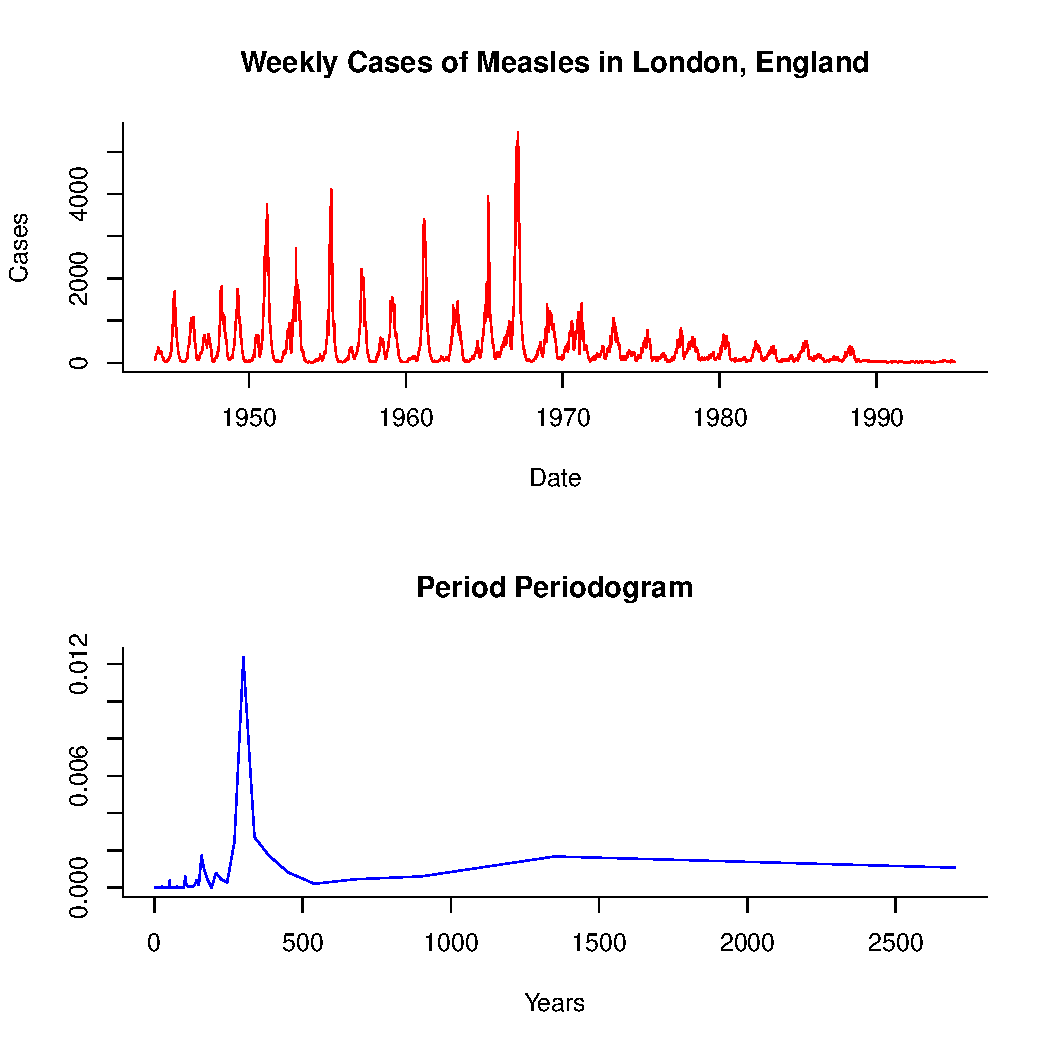
\includegraphics[width=\maxwidth]{figure/measlesplots-1} 
\begin{kframe}\begin{alltt}
\hlstd{lpl.data} \hlkwb{<-} \hlkwd{read.ymdc}\hlstd{(}\hlstr{"meas_uk__lpl_1944-94_wk.csv"}\hlstd{)}
\hlkwd{par}\hlstd{(}\hlkwc{mfrow}\hlstd{=}\hlkwd{c}\hlstd{(}\hlnum{2}\hlstd{,}\hlnum{1}\hlstd{))}
\hlkwd{time.plot}\hlstd{(lpl.data,} \hlkwc{ma.smooth}\hlstd{=}\hlnum{FALSE}\hlstd{,} \hlkwc{add}\hlstd{=}\hlnum{FALSE}\hlstd{,} \hlkwc{type}\hlstd{=}\hlstr{"l"}\hlstd{,} \hlkwc{xlab}\hlstd{=}\hlstr{"Date"}\hlstd{,} \hlkwc{ylab}\hlstd{=}\hlstr{"Cases"}\hlstd{,} \hlkwc{main}\hlstd{=}\hlstr{"Weekly Cases of Measles in Liverpool, England"}\hlstd{,} \hlkwc{bty}\hlstd{=}\hlstr{"l"}\hlstd{,} \hlkwc{col}\hlstd{=}\hlstr{"red"}\hlstd{)}
\hlkwd{periodogram}\hlstd{(lpl.data,} \hlkwc{add}\hlstd{=}\hlnum{FALSE}\hlstd{,} \hlkwc{type}\hlstd{=}\hlstr{"l"}\hlstd{,} \hlkwc{xlab}\hlstd{=}\hlstr{"Years"}\hlstd{,} \hlkwc{ylab}\hlstd{=}\hlstr{""}\hlstd{,} \hlkwc{main}\hlstd{=}\hlstr{"Period Periodogram"}\hlstd{,}\hlkwc{bty}\hlstd{=}\hlstr{"l"}\hlstd{,}\hlkwc{col}\hlstd{=}\hlstr{"blue"}\hlstd{)}
\end{alltt}
\end{kframe}
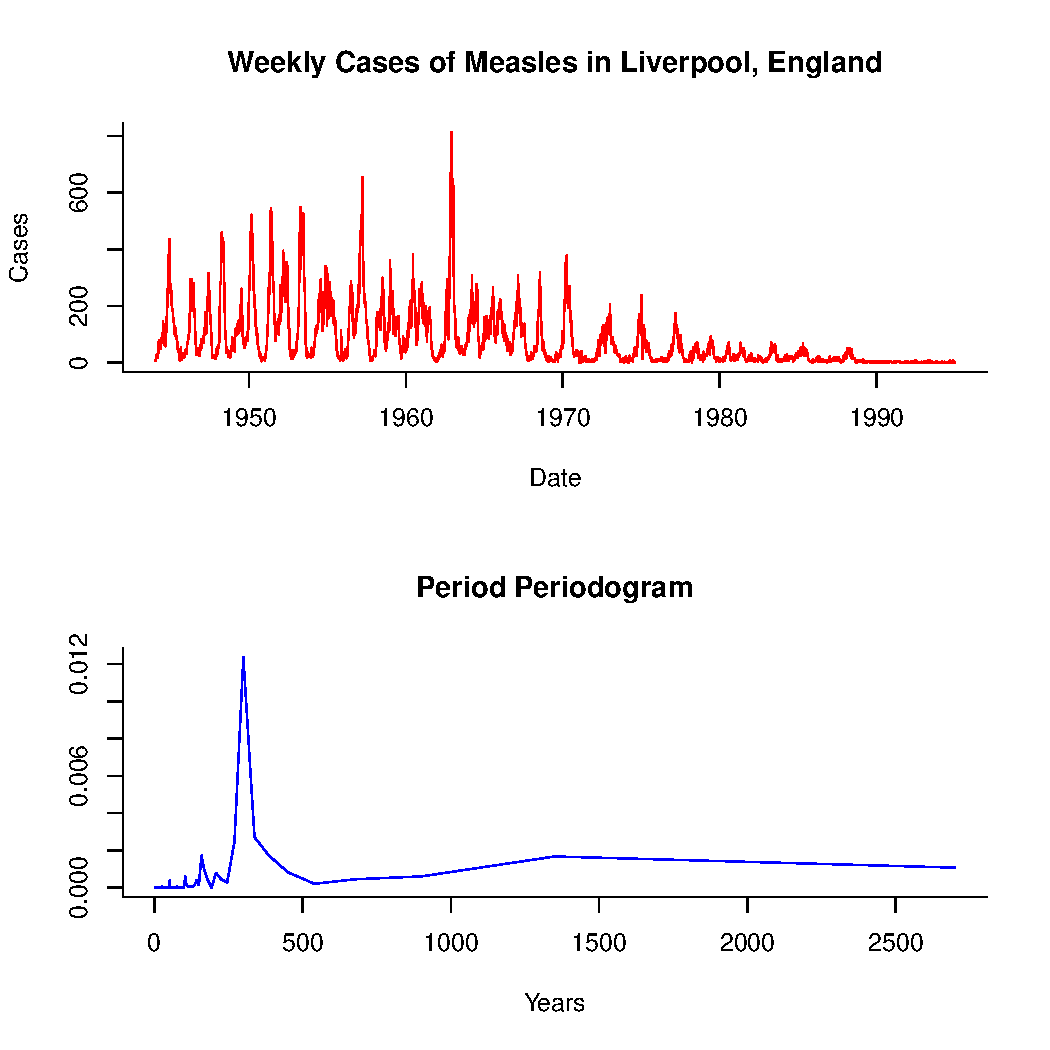
\includegraphics[width=\maxwidth]{figure/measlesplots-2} 

\end{knitrout}

}
\end{proof}
}

\end{enumerate}

\section{Stochastic Epidemic Simulations}

Consider the SI model,
%
\begin{equation}\label{E:SI}
  \frac{dI}{dt} = \beta (N-I) I \,, \qquad I(0)=I_0,
\end{equation}
%
where $\beta$ is the transmission rate, $N$ is the population size and
$I(t)$ is the number of infected individuals at time $t$.

\begin{enumerate}[(a)]

\item Write an \Rlogo function \magcode{SI.Gillespie()} that uses the
  Gillespie algorithm to produce a realization of a stochastic process
  whose mean field dynamics are given by equation \eqref{E:SI} in the
  limit $N\to\infty$.  Your function should have arguments
  \code{beta}, \code{N}, \code{I0} and \code{tmax} (the time at which
  to end the simulation).  You may find it helpful (conceptually) to write
  equation~\eqref{E:SI} in two-variable form:
  \begin{subequations}
    \begin{align}
      \frac{dS}{dt} &= -\beta S I \,, \qquad S(0)=N-I_0, \\
      \frac{dI}{dt} &= \beta S I \,, \qquad\quad I(0)=I_0.
    \end{align}
  \end{subequations}
  Note that there is only one type of event that can occur, so the second part of the Gillespie algorithm (what type of event occurred) is trivial for this model.
  
\emph{\underline{Note}:} To make stochastic simulations exactly reproducible use \texttt{\color{magenta}set.seed()}.

{\color{blue}
\begin{proof}[Solution]
{\color{magenta}
\begin{knitrout}
\definecolor{shadecolor}{rgb}{0.969, 0.969, 0.969}\color{fgcolor}\begin{kframe}
\begin{alltt}
\hlstd{SI.Gillespie} \hlkwb{<-} \hlkwa{function}\hlstd{(}\hlkwc{beta}\hlstd{,} \hlkwc{N}\hlstd{,} \hlkwc{I0}\hlstd{,} \hlkwc{tmax}\hlstd{)\{}
  \hlstd{timeseries} \hlkwb{<-} \hlkwd{c}\hlstd{()}
  \hlstd{timeseries} \hlkwb{<-} \hlkwd{rbind}\hlstd{(timeseries,} \hlkwd{c}\hlstd{(}\hlnum{0}\hlstd{,I0))}
  \hlstd{index} \hlkwb{<-} \hlnum{1}
  \hlkwa{while}\hlstd{(timeseries[index,}\hlnum{1}\hlstd{]} \hlopt{<} \hlstd{tmax)\{}
    \hlkwa{if} \hlstd{(timeseries[index,}\hlnum{2}\hlstd{]} \hlopt{<} \hlstd{N)\{}
      \hlstd{rate} \hlkwb{<-} \hlstd{beta}\hlopt{*}\hlstd{(timeseries[index,}\hlnum{2}\hlstd{])}\hlopt{*}\hlstd{(N}\hlopt{-}\hlstd{timeseries[index,}\hlnum{2}\hlstd{])}
      \hlstd{timestep} \hlkwb{<-} \hlkwd{rexp}\hlstd{(}\hlkwc{n}\hlstd{=}\hlnum{1}\hlstd{,} \hlkwc{rate}\hlstd{= rate)}
      \hlstd{timeseries} \hlkwb{<-} \hlkwd{rbind}\hlstd{(timeseries,} \hlkwd{c}\hlstd{(timeseries[index,}\hlnum{1}\hlstd{]}\hlopt{+}\hlstd{timestep, timeseries[index,}\hlnum{2}\hlstd{]}\hlopt{+}\hlnum{1}\hlstd{))}
    \hlstd{\}}\hlkwa{else}\hlstd{\{}
      \hlstd{timeseries} \hlkwb{<-} \hlkwd{rbind}\hlstd{(timeseries,} \hlkwd{c}\hlstd{(timeseries[index,}\hlnum{1}\hlstd{]}\hlopt{+}\hlstd{timestep}\hlopt{*}\hlnum{3}\hlstd{, timeseries[index,}\hlnum{2}\hlstd{]))}
    \hlstd{\}}
    \hlstd{index} \hlkwb{<-} \hlstd{index}\hlopt{+}\hlnum{1}
  \hlstd{\}}
  \hlkwd{return}\hlstd{(timeseries)}
\hlstd{\}}
\end{alltt}
\end{kframe}
\end{knitrout}


}
\end{proof}
}

\item Make a multi-panel plot comparing the deterministic and stochastic dynamics of the SI model for $\beta=1$, $I_0=1$ and $N\in\{32,10^2,10^3,10^4\}$ ($N=32$ is close to $10^{1.5}$).  Each panel should correspond to a different value of $N$ and should show 30 stochastic realizations together with the deterministic solution.

{\color{blue}
\begin{proof}[Solution]
{\color{magenta}
\begin{knitrout}
\definecolor{shadecolor}{rgb}{0.969, 0.969, 0.969}\color{fgcolor}\begin{kframe}
\begin{alltt}
\hlcom{## Vector Field for SI model}
\hlstd{SI.vector.field} \hlkwb{<-} \hlkwa{function}\hlstd{(}\hlkwc{t}\hlstd{,} \hlkwc{vars}\hlstd{,} \hlkwc{parms}\hlstd{=}\hlkwd{c}\hlstd{(}\hlkwc{beta}\hlstd{=}\hlnum{2}\hlstd{,}\hlkwc{gamma}\hlstd{=}\hlnum{1}\hlstd{)) \{}
  \hlkwd{with}\hlstd{(}\hlkwd{as.list}\hlstd{(}\hlkwd{c}\hlstd{(parms, vars)), \{}
    \hlstd{dx} \hlkwb{<-} \hlopt{-}\hlstd{beta}\hlopt{*}\hlstd{x}\hlopt{*}\hlstd{y} \hlcom{# dS/dt}
    \hlstd{dy} \hlkwb{<-} \hlstd{beta}\hlopt{*}\hlstd{x}\hlopt{*}\hlstd{y}  \hlcom{# dI/dt}
    \hlstd{vec.fld} \hlkwb{<-} \hlkwd{c}\hlstd{(}\hlkwc{dx}\hlstd{=dx,} \hlkwc{dy}\hlstd{=dy)}
    \hlkwd{return}\hlstd{(}\hlkwd{list}\hlstd{(vec.fld))} \hlcom{# ode() requires a list}
  \hlstd{\})}
\hlstd{\}}
\end{alltt}
\end{kframe}
\end{knitrout}

\begin{knitrout}
\definecolor{shadecolor}{rgb}{0.969, 0.969, 0.969}\color{fgcolor}\begin{kframe}
\begin{alltt}
\hlcom{## Draw solution}
\hlkwd{library}\hlstd{(}\hlstr{"deSolve"}\hlstd{)}
\hlstd{draw.soln} \hlkwb{<-} \hlkwa{function}\hlstd{(}\hlkwc{ic}\hlstd{=}\hlkwd{c}\hlstd{(}\hlkwc{x}\hlstd{=}\hlnum{1}\hlstd{,}\hlkwc{y}\hlstd{=}\hlnum{0}\hlstd{),} \hlkwc{tmax}\hlstd{=}\hlnum{1}\hlstd{,}
                      \hlkwc{times}\hlstd{=}\hlkwd{seq}\hlstd{(}\hlnum{0}\hlstd{,tmax,}\hlkwc{by}\hlstd{=tmax}\hlopt{/}\hlnum{500}\hlstd{),}
                      \hlkwc{func}\hlstd{,} \hlkwc{parms}\hlstd{,} \hlkwc{...} \hlstd{) \{}
  \hlstd{soln} \hlkwb{<-} \hlkwd{ode}\hlstd{(ic, times, func, parms)}
  \hlkwd{lines}\hlstd{(times, soln[,}\hlstr{"y"}\hlstd{],} \hlkwc{col}\hlstd{=}\hlstr{"blue"}\hlstd{,} \hlkwc{lwd}\hlstd{=}\hlnum{3}\hlstd{, ... )}
\hlstd{\}}
\end{alltt}
\end{kframe}
\end{knitrout}

\begin{knitrout}
\definecolor{shadecolor}{rgb}{0.969, 0.969, 0.969}\color{fgcolor}\begin{kframe}
\begin{alltt}
\hlstd{beta} \hlkwb{<-} \hlnum{1}
\hlstd{I0} \hlkwb{<-} \hlnum{1}
\hlstd{tmax} \hlkwb{<-} \hlnum{0.3}
\hlstd{N} \hlkwb{<-} \hlkwd{c}\hlstd{(}\hlnum{32}\hlstd{,} \hlnum{10}\hlopt{^}\hlnum{2}\hlstd{,} \hlnum{10}\hlopt{^}\hlnum{3}\hlstd{,} \hlnum{10}\hlopt{^}\hlnum{4}\hlstd{)}

\hlkwd{par}\hlstd{(}\hlkwc{mfrow}\hlstd{=}\hlkwd{c}\hlstd{(}\hlkwd{length}\hlstd{(N),}\hlnum{1}\hlstd{))}
\hlkwa{for} \hlstd{(j} \hlkwa{in} \hlnum{1}\hlopt{:}\hlkwd{length}\hlstd{(N))\{}
  \hlcom{## draw box for plot}
  \hlkwd{plot}\hlstd{(}\hlnum{0}\hlstd{,}\hlnum{0}\hlstd{,}\hlkwc{xlim}\hlstd{=}\hlkwd{c}\hlstd{(}\hlnum{0}\hlstd{,tmax),}\hlkwc{ylim}\hlstd{=}\hlkwd{c}\hlstd{(}\hlnum{0}\hlstd{,N[j]}\hlopt{+}\hlnum{1}\hlstd{),}\hlkwc{xlab}\hlstd{=}\hlstr{"Time"}\hlstd{,} \hlkwc{ylab}\hlstd{=}\hlstr{"Prevalence (I)"}\hlstd{,} \hlkwc{main}\hlstd{=}\hlkwd{paste}\hlstd{(}\hlstr{"$\textbackslash{}\textbackslash{}N ="}\hlstd{, N[j]))}
  \hlstd{line} \hlkwb{<-} \hlkwd{c}\hlstd{(}\hlnum{1}\hlopt{:}\hlnum{30}\hlstd{)}
  \hlkwa{for} \hlstd{(i} \hlkwa{in} \hlnum{1}\hlopt{:}\hlkwd{length}\hlstd{(line)) \{}
    \hlkwd{set.seed}\hlstd{(line[i])}
    \hlkwd{lines}\hlstd{(}\hlkwd{SI.Gillespie}\hlstd{(beta, N[j], I0, tmax),}\hlkwc{lty}\hlstd{=}\hlstr{"dotted"}\hlstd{,}
            \hlkwc{col}\hlstd{=line[i}\hlopt{+}\hlnum{1}\hlstd{])} \hlcom{# use a different line colour for each solution}
  \hlstd{\}}
  \hlkwd{draw.soln}\hlstd{(}\hlkwc{ic}\hlstd{=}\hlkwd{c}\hlstd{(}\hlkwc{x}\hlstd{=N[j]}\hlopt{-}\hlstd{I0,}\hlkwc{y}\hlstd{=I0),} \hlkwc{tmax}\hlstd{=tmax,}
            \hlkwc{func}\hlstd{= SI.vector.field,}
            \hlkwc{parms}\hlstd{=}\hlkwd{c}\hlstd{(beta,}\hlkwc{gamma}\hlstd{=}\hlnum{1}\hlstd{))}
\hlstd{\}}
\end{alltt}
\end{kframe}
\end{knitrout}

}
\end{proof}
}

\end{enumerate}

\section{$\R_0$ for smallpox}

The natural history of smallpox is shown in \fref{smpxnathist}.  The US Centers for Disease Control and Prevention (CDC) has recently discovered that a group of bioterrorists plans to reintroduce smallpox to the United States.  The CDC has reason to believe that the terrorists are also bioengineers and have successfully altered the virus so that it causes the early rash stage to be twice as long as it was when the virus was last circulating naturally in the 1970s.  Moreover, the existing smallpox vaccine apparently provides no protection against the altered virus.  The CDC wants your opinion on how the alterations to the virus will affect $\R_0$ and the expected final size of an epidemic if the planned attack is successful.

\begin{enumerate}[(a)]
  \item Construct a compartmental (ODE) smallpox transmission model based on the natural history specified in \fref{smpxnathist}, including vital dynamics but ignoring disease-induced death.

{\color{blue}
\begin{proof}[Solution]
{\color{magenta}
A compartmental (ODE) smallpox transmission model based on the natural history and assuming time spent in each stage of the disease is expontentially distributed is given by
\begin{center}
{\color{black}
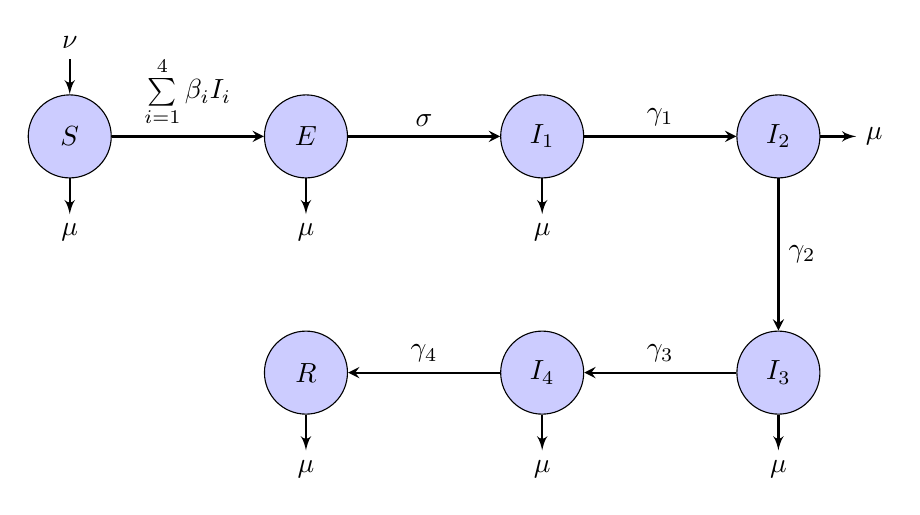
\begin{tikzpicture}[node distance=3cm,auto,>=latex',every node/.append style={align=center}]
    \node [int, pin={[pinstyleto]above:$\nu$}, pin={[pinstyleout]below:$\mu$}] (a)              {$S$};
    \node [int, pin={[pinstyleout]below:$\mu$}] (b) [right of=a] {$E$};
    \node [int, pin={[pinstyleout]below:$\mu$}] (c) [right of=b] {$I_1$};
    \node [int, pin={[pinstyleout]right:$\mu$}] (d) [right of=c] {$I_2$};
    \node [int, pin={[pinstyleout]below:$\mu$}] (e) [below of=d] {$I_3$};
    \node [int, pin={[pinstyleout]below:$\mu$}] (f) [left of=e] {$I_4$};
    \node [int, pin={[pinstyleout]below:$\mu$}] (g) [left of=f] {$R$};
    \draw [arrow] (a) -- node[anchor=south] {$ \sum\limits_{i=1}^{4}\beta_i I_i $} (b);
    \draw [arrow] (b) -- node[anchor=south] {$\sigma$} (c);
    \draw [arrow] (c) -- node[anchor=south] {$\gamma_1$} (d);
    \draw [arrow] (d) -- node[anchor=west] {$\gamma_2$} (e);
    \draw [arrow] (e) -- node[anchor=south] {$\gamma_3$} (f);
    \draw [arrow] (f) -- node[anchor=south] {$\gamma_4$} (g);                                  
\end{tikzpicture}
}
\end{center}

\begin{align}
  \frac{dS}{dt} &= \nu - S\sum\limits_{i=1}^{4}\beta_i I_i -\mu S \\ 
  \frac{dE}{dt} &= S\sum\limits_{i=1}^{4}\beta_i I_i -\sigma E - \mu E \\
  \frac{dI_1}{dt} &= \sigma E - \gamma_1 I_1 -\mu I_1 \\
  \dots \\
  \frac{dI_i}{dt} &= \gamma_{i-1} I_{i-1} -\gamma_{i} I_{i} -\mu I_{i} , \quad \quad 0<i\leq 4\\
  \dots \\
  \frac{dR}{dt} &= \gamma_5 I_5 -\mu R 
\end{align}

The notation of the compartments is as follows
\begin{center}
\begin{tabular}{ l | l }
  Notation & Definition \\
  \hline			
  $S$ & Proportion of population that is susceptible \\
  $E$ & Proportion of population in the incubation stage \\
  $I_1$ & Proportion of population in the prodrom stage \\
  $I_2$ & Proportion of population in the early rash stage \\
  $I_3$ & Proportion of population in the pustular rash stage \\
  $I_4$ & Proportion of population in the scarbs stage \\
  $R$ & Proportion of population that is recovered\\
  \hline  
\end{tabular}
\end{center}

The notation of the rates and waiting times is as follows
\begin{center}
\begin{tabular}{ l | l | l }
  Notation & Definition & Value for original virus \\
  \hline			
  $\nu$ & Birth rate & \\
  $\beta_i$ & Transmission rate due to individuals from compartment $I_i$ &  \\
  $\frac{1}{\sigma}$ & Mean time spent in compartment $E$ & 12 days \\
  $\frac{1}{\gamma_1}$ & Mean time spent in compartment $I_1$ &  3 days \\
  $\frac{1}{\gamma_2}$ & Mean time spent in compartment $I_2$ & 4 days \\
  $\frac{1}{\gamma_3}$ & Mean time spent in compartment $I_3$ & 5 days  \\
  $\frac{1}{\gamma_4}$ & Mean time spent in compartment $I_4$ & 11 days \\
  $\mu$ & Death rate\\
  \hline  
\end{tabular}
\end{center}

}
\end{proof}
}

  \item Use a biological argument to find a formula for $\R_0$.

{\color{blue}
\begin{proof}[Solution]
{\color{magenta}\dots beautifully clear and concise text to be inserted here\dots}
\end{proof}
}

  \item Calculate $\R_0$ using the next generation matrix approach.  \emph{\underline{Note}:} Your solution should include $\mathcal F$, $\mathcal V$, $F$, $V$, and $FV^{-1}$, in the most human-friendly form you can find.  However, feel free to use symbolic manipulation software such as \texttt{Maple}, {\slshape Mathematica\/} or \href{http://www.sagemath.org/}{sage} to help with the necessary algebra and matrix computations.

{\color{blue}
\begin{proof}[Solution]
{\color{magenta}

\[
\frac{d}{dt}
\begin{bmatrix}
  E \\
  I_1 \\
  I_2 \\
  I_3 \\
  I_4
\end{bmatrix}
=
\begin{bmatrix}
  S\sum\limits_{i=1}^{4}\beta_i I_i - \sigma E - \mu E \\
  \sigma E - \gamma_1 I_1 -\mu I_1 \\
  \gamma_{1} I_{1} -\gamma_{2} I_{2} -\mu I_{2} \\
  \gamma_{2} I_{2} -\gamma_{3} I_{3} -\mu I_{3} \\
  \gamma_{3} I_{3} -\gamma_{4} I_{4} -\mu I_{4} 
\end{bmatrix}
\\
= \mathcal{F} - \mathcal{V}
\]

\[
\mathcal{F}= \text{The inflow of new infected into infected compartments} \\
=
\begin{bmatrix}
  S\sum\limits_{i=1}^{4}\beta_i I_i \\
  0 \\
  0 \\
  0 \\
  0 
\end{bmatrix}
\]
\[
\mathcal{V}= \text{The outflow of from infected compartments} \\
=
\begin{bmatrix}
  \sigma E + \mu E \\
  -\sigma E + \gamma_1 I_1 +\mu I_1 \\
  -\gamma_{1} I_{1} +\gamma_{2} I_{2} +\mu I_{2} \\
  -\gamma_{2} I_{2} +\gamma_{3} I_{3} +\mu I_{3} \\
  -\gamma_{3} I_{3} +\gamma_{4} I_{4} +\mu I_{4} 
\end{bmatrix}
\]
The Jacobians of these vectors at the disease free equilibrium, $(S^*,I_1^*,\dots,I_4^*)=(1,0, \dots, 0)$, are
\[
F = D\mathcal{F}_{(S^*,I_i^*)} \\
=
\begin{bmatrix}
  0 & \beta_1 & \beta_2 & \beta_3 & \beta_4 \\
  0 & 0 & 0 & 0 & 0 \\
  0 & 0 & 0 & 0 & 0 \\
  0 & 0 & 0 & 0 & 0 \\
  0 & 0 & 0 & 0 & 0 
\end{bmatrix}
\]

\[
V = D\mathcal{V}_{(S^*,I_i^*)} \\
= \begin{bmatrix}
  \sigma + \mu & 0 & 0 & 0 & 0 \\
  -\sigma & \gamma_1+\mu & 0 & 0 & 0\\
  0 & -\gamma_1 & \gamma_2+\mu & 0 & 0 \\
  0 & 0 & -\gamma_2 & \gamma_3+\mu & 0 \\
  0 & 0 & 0 & -\gamma_3 & \gamma_4+\mu 
\end{bmatrix}
\]
The inverse of $V$ is
\[
V^{-1}= 
\begin{bmatrix}
  \frac{1}{\sigma + \mu} & 0 & 0 & 0 & 0 \\
  \frac{\sigma}{(\sigma + \mu)(\gamma_1+\mu)} & \frac{1}{\gamma_1+\mu} & 0 & 0 & 0\\
  
  \frac{\sigma \gamma_1}{(\sigma + \mu)(\gamma_1+\mu)(\gamma_2+\mu)} & \frac{\gamma_1}{(\gamma_1+\mu)(\gamma_2+\mu)} & \frac{1}{\gamma_2+\mu} & 0 & 0 \\
  
  \frac{\sigma \gamma_1 \gamma_2}{(\sigma + \mu)(\gamma_1+\mu)(\gamma_2+\mu)(\gamma_3+\mu)} & \frac{\gamma_1 \gamma_2}{(\gamma_1+\mu)(\gamma_2+\mu)(\gamma_3+\mu)} & \frac{\gamma_2}{(\gamma_2+\mu)(\gamma_3+\mu)} & \frac{1}{\gamma_3+\mu} & 0 \\
  
  \frac{\sigma \gamma_1 \gamma_2 \gamma_3}{(\sigma + \mu)(\gamma_1+\mu)(\gamma_2+\mu)(\gamma_3+\mu)(\gamma_4+\mu)} & \frac{\gamma_1 \gamma_2 \gamma_3}{(\gamma_1+\mu)(\gamma_2+\mu)(\gamma_3+\mu)(\gamma_4+\mu)} & \frac{\gamma_2 \gamma_3}{(\gamma_2+\mu)(\gamma_3+\mu)(\gamma_4+\mu)} & \frac{\gamma_3}{(\gamma_3+\mu)(\gamma_4+\mu)} & \frac{1}{\gamma_4+\mu} 
\end{bmatrix}
\]
The next generation matrix (computed using Mathematica) is 
\[
FV^{-1}= 
\begin{bmatrix}
  & & A^T
  \\
  0 & 0 & 0 & 0 & 0 \\
  0 & 0 & 0 & 0 & 0 \\
  0 & 0 & 0 & 0 & 0 \\
  0 & 0 & 0 & 0 & 0 
\end{bmatrix}
\]
where 
\[
A = 
\begin{bmatrix}
  \frac{\sigma}{(\sigma + \mu)(\gamma_1+\mu)} \left ( \beta_1 + \frac{\beta_2 \gamma_1}{\gamma_2+\mu} + \frac{\beta_3 \gamma_1\gamma_2}{(\gamma_2+\mu)(\gamma_3+\mu)} + \frac{\beta_4 \gamma_1\gamma_2\gamma_3}{(\gamma_2+\mu)(\gamma_3+\mu)(\gamma_4+\mu)} \right )
  \\ 
  \frac{1}{\gamma_1+\mu} \left ( \beta_1 + \frac{\beta_2 \gamma_1}{\gamma_2+\mu} + \frac{\beta_3 \gamma_1\gamma_2}{(\gamma_2+\mu)(\gamma_3+\mu)} + \frac{\beta_4 \gamma_1\gamma_2\gamma_3}{(\gamma_2+\mu)(\gamma_3+\mu)(\gamma_4+\mu)} \right )
  \\ 
  \frac{1}{\gamma_2+\mu} \left ( \beta_2 + \frac{\beta_3 \gamma_2}{\gamma_3+\mu} + \frac{\beta_4 \gamma_2\gamma_3}{(\gamma_3+\mu)(\gamma_4+\mu)}  \right )
  \\
  \frac{1}{\gamma_3+\mu} \left ( \beta_3  + \frac{\beta_4 \gamma_3}{\gamma_4+\mu}  \right )
  \\
  \frac{\beta_4}{\gamma_4+\mu}

\end{bmatrix}
\]

$\R_0$ is the spectral radius - i.e. the maximum eigenvalue - of this matrix. Using Mathematica to compute this:
\begin{align}
  \R_0 &= \rho (FV^{-1}) \\
  &= \frac{\sigma}{(\sigma + \mu)(\gamma_1+\mu)(\gamma_2+\mu)} \left ( \beta_1(\gamma_2+\mu) + \frac{\beta_2\gamma_1(\gamma_3+\mu)}{\gamma_3+\mu}
+ \frac{\beta_3\gamma_1\gamma_2(\gamma_4+\mu)}{(\gamma_3+\mu)(\gamma_4+\mu)}
+ \frac{\beta_4\gamma_1\gamma_2\gamma_3}{(\gamma_3+\mu)(\gamma_4+\mu)}
  \right ) \\
  &= \frac{\sigma}{(\sigma + \mu)(\gamma_1+\mu)(\gamma_2+\mu)(\gamma_3+\mu)(\gamma_4+\mu)} ( \beta_1(\gamma_2+\mu)(\gamma_3+\mu)(\gamma_4+\mu) \nonumber \\
  & + \beta_2\gamma_1(\gamma_3+\mu)(\gamma_4+\mu) +\beta_3\gamma_1\gamma_2(\gamma_4+\mu) +\beta_4\gamma_1\gamma_2\gamma_3
   )
\end{align}


}
\end{proof}
}

  \item Based on your model, and $\R_0\sim5$ for unaltered smallpox, what can you say about the difference in $\R_0$ that can be expected for the newly engineered virus vs.\ the original virus?  

{\color{blue}
\begin{proof}[Solution]
{\color{magenta}
Let $\tilde{\R_0}$ be the value of $\R_0$ for the newly engineered virus. All of the parameters are the same as for unaltered smallpox except $\frac{1}{\tilde{\gamma_2}}=\frac{2}{\gamma_2}$. 
}
\end{proof}
}

\item Write a paragraph that you can imagine e-mailing to the CDC, in which you do your best to answer their questions.
\end{enumerate}

{\color{blue}
\begin{proof}[Solution]
{\color{magenta}\dots beautifully clear and concise text to be inserted here\dots}
\end{proof}
}

%
\begin{figure}[h]
\begin{center}
\scalebox{1}{
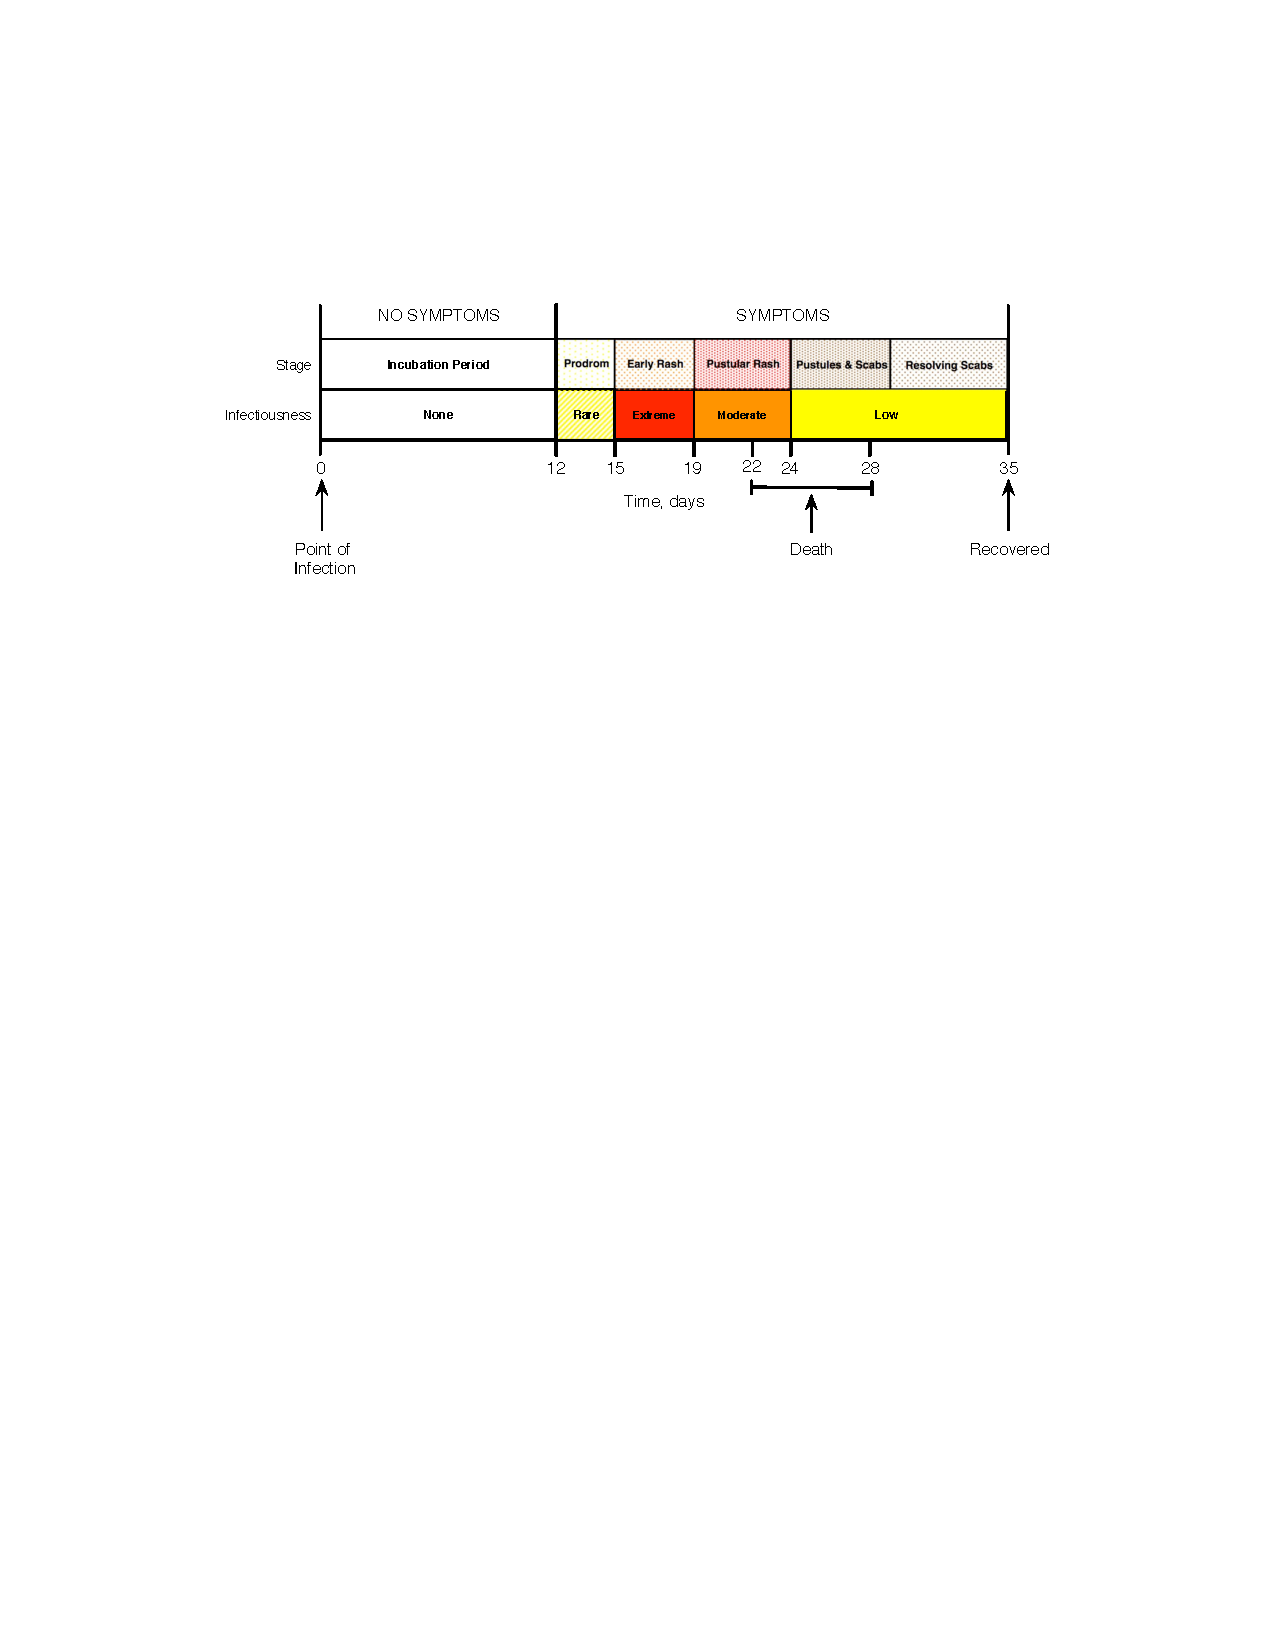
\includegraphics{smpxnathist_p82.pdf}
}
\end{center}
\caption{The natural history of smallpox infection. The prodrom stage begins with fever but the patient is very rarely contagious. Early rash is the most contagious stage, when the rash develops and transforms into bumps. During the pustular rash stage bumps become pustules, which then turn into scabs during the pustules and scabs stage and fall off during the resolving scabs stage. The infected person is contagious until the last scab falls off.  (\emph{This is Figure 3.4 from page 82 of Olga Krylova's 2011 McMaster University PhD thesis.})}
\label{F:smpxnathist}
\end{figure}
%

\bigskip
\centerline{\bf--- END OF ASSIGNMENT ---}

\bigskip
Compile time for this document:
\today\ @ \thistime

\end{document}
